

\tikzset{every picture/.style={line width=0.75pt}} %set default line width to 0.75pt        

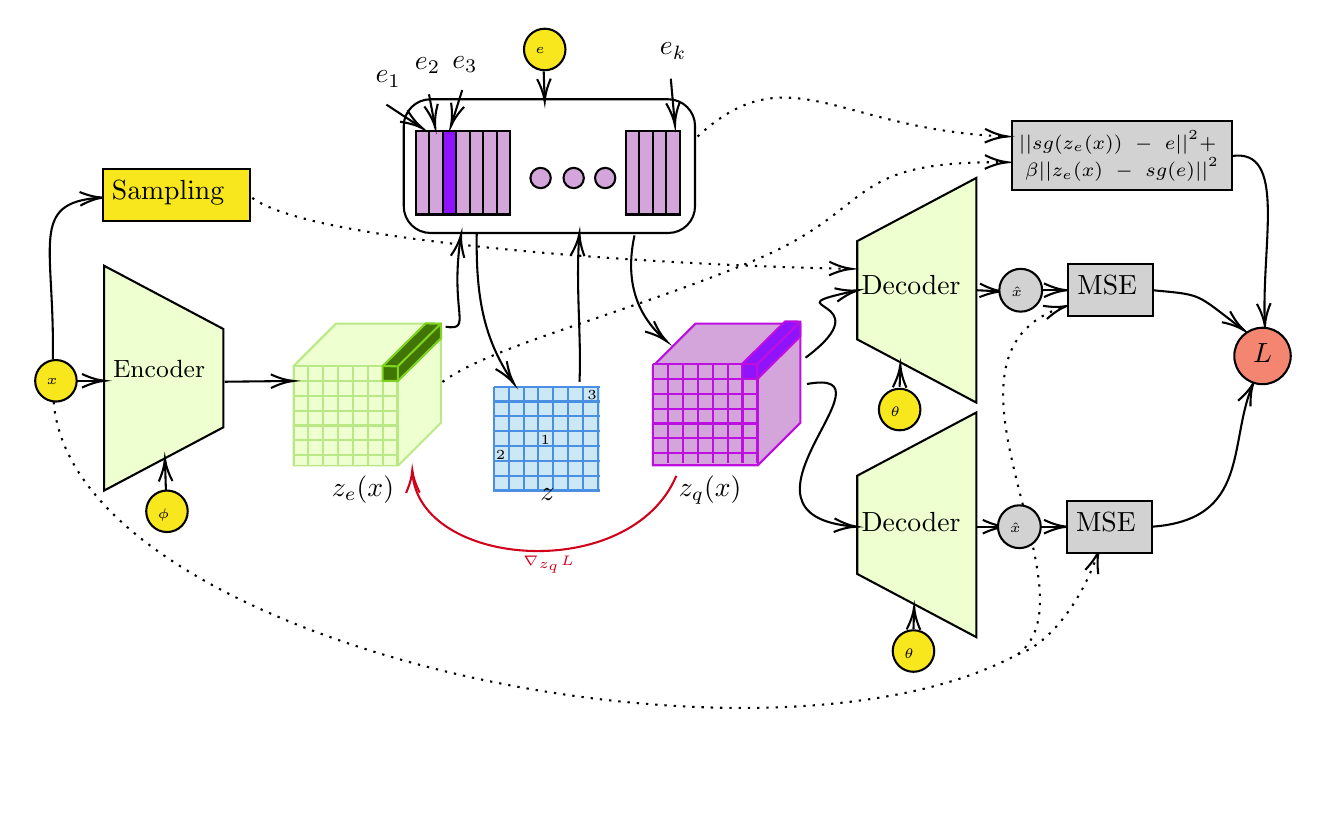
\begin{tikzpicture}[x=0.75pt,y=0.75pt,yscale=-1,xscale=1]
%uncomment if require: \path (0,308); %set diagram left start at 0, and has height of 308

%Shape: Trapezoid [id:dp9970991985728426] 
\draw  [fill={rgb, 255:red, 238; green, 255; blue, 208 }  ,fill opacity=1 ] (97.75,141.72) -- (155.17,172.18) -- (155.17,219.54) -- (97.75,250) -- cycle ;
%Shape: Cube [id:dp42361480595854006] 
\draw  [color={rgb, 255:red, 184; green, 233; blue, 134 }  ,draw opacity=1 ][fill={rgb, 255:red, 238; green, 255; blue, 208 }  ,fill opacity=1 ] (189,190.06) -- (209.47,169.59) -- (260,169.59) -- (260,217.36) -- (239.53,237.83) -- (189,237.83) -- cycle ; \draw  [color={rgb, 255:red, 184; green, 233; blue, 134 }  ,draw opacity=1 ] (260,169.59) -- (239.53,190.06) -- (189,190.06) ; \draw  [color={rgb, 255:red, 184; green, 233; blue, 134 }  ,draw opacity=1 ] (239.53,190.06) -- (239.53,237.83) ;
%Shape: Grid [id:dp7309056371427156] 
\draw  [draw opacity=0][fill={rgb, 255:red, 238; green, 255; blue, 208 }  ,fill opacity=1 ][line width=0.75]  (189,190.06) -- (239.36,190.06) -- (239.36,237.83) -- (189,237.83) -- cycle ; \draw  [color={rgb, 255:red, 184; green, 233; blue, 134 }  ,draw opacity=1 ][line width=0.75]  (189,190.06) -- (189,237.83)(196.15,190.06) -- (196.15,237.83)(203.3,190.06) -- (203.3,237.83)(210.45,190.06) -- (210.45,237.83)(217.6,190.06) -- (217.6,237.83)(224.75,190.06) -- (224.75,237.83)(231.9,190.06) -- (231.9,237.83)(239.05,190.06) -- (239.05,237.83) ; \draw  [color={rgb, 255:red, 184; green, 233; blue, 134 }  ,draw opacity=1 ][line width=0.75]  (189,190.06) -- (239.36,190.06)(189,197.21) -- (239.36,197.21)(189,204.36) -- (239.36,204.36)(189,211.51) -- (239.36,211.51)(189,218.66) -- (239.36,218.66)(189,225.81) -- (239.36,225.81)(189,232.96) -- (239.36,232.96) ; \draw  [color={rgb, 255:red, 184; green, 233; blue, 134 }  ,draw opacity=1 ][line width=0.75]   ;
%Shape: Cube [id:dp22785524738202734] 
\draw  [color={rgb, 255:red, 126; green, 211; blue, 33 }  ,draw opacity=1 ][fill={rgb, 255:red, 65; green, 117; blue, 5 }  ,fill opacity=1 ] (231.89,190.05) -- (252.68,169.48) -- (260,169.59) -- (260.03,176.67) -- (239.25,197.24) -- (231.92,197.13) -- cycle ; \draw  [color={rgb, 255:red, 126; green, 211; blue, 33 }  ,draw opacity=1 ] (260,169.59) -- (239.22,190.16) -- (231.89,190.05) ; \draw  [color={rgb, 255:red, 126; green, 211; blue, 33 }  ,draw opacity=1 ] (239.22,190.16) -- (239.25,197.24) ;
%Shape: Grid [id:dp6272744783093117] 
\draw  [draw opacity=0][fill={rgb, 255:red, 204; green, 232; blue, 244 }  ,fill opacity=1 ][line width=0.75]  (285.5,199.95) -- (336.5,199.95) -- (336.5,250.95) -- (285.5,250.95) -- cycle ; \draw  [color={rgb, 255:red, 74; green, 144; blue, 226 }  ,draw opacity=1 ][line width=0.75]  (285.5,199.95) -- (285.5,250.95)(292.65,199.95) -- (292.65,250.95)(299.8,199.95) -- (299.8,250.95)(306.95,199.95) -- (306.95,250.95)(314.1,199.95) -- (314.1,250.95)(321.25,199.95) -- (321.25,250.95)(328.4,199.95) -- (328.4,250.95)(335.55,199.95) -- (335.55,250.95) ; \draw  [color={rgb, 255:red, 74; green, 144; blue, 226 }  ,draw opacity=1 ][line width=0.75]  (285.5,199.95) -- (336.5,199.95)(285.5,207.1) -- (336.5,207.1)(285.5,214.25) -- (336.5,214.25)(285.5,221.4) -- (336.5,221.4)(285.5,228.55) -- (336.5,228.55)(285.5,235.7) -- (336.5,235.7)(285.5,242.85) -- (336.5,242.85)(285.5,250) -- (336.5,250) ; \draw  [color={rgb, 255:red, 74; green, 144; blue, 226 }  ,draw opacity=1 ][line width=0.75]   ;
%Shape: Cube [id:dp809301632956687] 
\draw  [color={rgb, 255:red, 189; green, 16; blue, 224 }  ,draw opacity=1 ][fill={rgb, 255:red, 212; green, 165; blue, 219 }  ,fill opacity=1 ] (362.17,190.06) -- (382.64,169.59) -- (433.17,169.59) -- (433.17,217.36) -- (412.69,237.83) -- (362.17,237.83) -- cycle ; \draw  [color={rgb, 255:red, 189; green, 16; blue, 224 }  ,draw opacity=1 ] (433.17,169.59) -- (412.69,190.06) -- (362.17,190.06) ; \draw  [color={rgb, 255:red, 189; green, 16; blue, 224 }  ,draw opacity=1 ] (412.69,190.06) -- (412.69,237.83) ;
%Shape: Grid [id:dp8763656364690284] 
\draw  [draw opacity=0][fill={rgb, 255:red, 212; green, 165; blue, 219 }  ,fill opacity=1 ][line width=0.75]  (362.37,189.11) -- (412.73,189.11) -- (412.73,236.88) -- (362.37,236.88) -- cycle ; \draw  [color={rgb, 255:red, 189; green, 16; blue, 224 }  ,draw opacity=1 ][line width=0.75]  (362.37,189.11) -- (362.37,236.88)(369.52,189.11) -- (369.52,236.88)(376.67,189.11) -- (376.67,236.88)(383.82,189.11) -- (383.82,236.88)(390.97,189.11) -- (390.97,236.88)(398.12,189.11) -- (398.12,236.88)(405.27,189.11) -- (405.27,236.88)(412.42,189.11) -- (412.42,236.88) ; \draw  [color={rgb, 255:red, 189; green, 16; blue, 224 }  ,draw opacity=1 ][line width=0.75]  (362.37,189.11) -- (412.73,189.11)(362.37,196.26) -- (412.73,196.26)(362.37,203.41) -- (412.73,203.41)(362.37,210.56) -- (412.73,210.56)(362.37,217.71) -- (412.73,217.71)(362.37,224.86) -- (412.73,224.86)(362.37,232.01) -- (412.73,232.01) ; \draw  [color={rgb, 255:red, 189; green, 16; blue, 224 }  ,draw opacity=1 ][line width=0.75]   ;
%Rounded Rect [id:dp16021058358844698] 
\draw   (242.08,74.38) .. controls (242.08,67.27) and (247.85,61.5) .. (254.97,61.5) -- (369.53,61.5) .. controls (376.65,61.5) and (382.42,67.27) .. (382.42,74.38) -- (382.42,113.03) .. controls (382.42,120.15) and (376.65,125.92) .. (369.53,125.92) -- (254.97,125.92) .. controls (247.85,125.92) and (242.08,120.15) .. (242.08,113.03) -- cycle ;
%Shape: Rectangle [id:dp15210766862939007] 
\draw  [fill={rgb, 255:red, 212; green, 165; blue, 219 }  ,fill opacity=1 ] (247.83,76.83) -- (254.33,76.83) -- (254.33,117) -- (247.83,117) -- cycle ;
%Shape: Rectangle [id:dp13078807954545157] 
\draw  [fill={rgb, 255:red, 212; green, 165; blue, 219 }  ,fill opacity=1 ] (254.33,76.83) -- (260.83,76.83) -- (260.83,117) -- (254.33,117) -- cycle ;
%Shape: Rectangle [id:dp6180191163450066] 
\draw  [fill={rgb, 255:red, 144; green, 19; blue, 254 }  ,fill opacity=1 ] (260.83,76.83) -- (267.33,76.83) -- (267.33,117) -- (260.83,117) -- cycle ;
%Shape: Rectangle [id:dp6007086788295256] 
\draw  [fill={rgb, 255:red, 212; green, 165; blue, 219 }  ,fill opacity=1 ] (267.33,76.83) -- (273.83,76.83) -- (273.83,117) -- (267.33,117) -- cycle ;
%Shape: Rectangle [id:dp8334769615864425] 
\draw  [fill={rgb, 255:red, 212; green, 165; blue, 219 }  ,fill opacity=1 ] (273.83,76.83) -- (280.33,76.83) -- (280.33,117) -- (273.83,117) -- cycle ;
%Shape: Rectangle [id:dp10885978237838678] 
\draw  [fill={rgb, 255:red, 212; green, 165; blue, 219 }  ,fill opacity=1 ] (280.33,76.83) -- (286.83,76.83) -- (286.83,117) -- (280.33,117) -- cycle ;
%Shape: Rectangle [id:dp791587758800796] 
\draw  [fill={rgb, 255:red, 212; green, 165; blue, 219 }  ,fill opacity=1 ] (286.83,76.83) -- (293.33,76.83) -- (293.33,117) -- (286.83,117) -- cycle ;
%Shape: Rectangle [id:dp7351728153510088] 
\draw  [fill={rgb, 255:red, 212; green, 165; blue, 219 }  ,fill opacity=1 ] (349,76.83) -- (355.5,76.83) -- (355.5,117) -- (349,117) -- cycle ;
%Shape: Rectangle [id:dp4641489804546418] 
\draw  [fill={rgb, 255:red, 212; green, 165; blue, 219 }  ,fill opacity=1 ] (355.5,76.83) -- (362,76.83) -- (362,117) -- (355.5,117) -- cycle ;
%Shape: Rectangle [id:dp1581276472212214] 
\draw  [fill={rgb, 255:red, 212; green, 165; blue, 219 }  ,fill opacity=1 ] (362,76.83) -- (368.5,76.83) -- (368.5,117) -- (362,117) -- cycle ;
%Shape: Rectangle [id:dp4957555362723687] 
\draw  [fill={rgb, 255:red, 212; green, 165; blue, 219 }  ,fill opacity=1 ] (368.5,76.83) -- (375,76.83) -- (375,117) -- (368.5,117) -- cycle ;
%Shape: Circle [id:dp4798210889469392] 
\draw  [fill={rgb, 255:red, 212; green, 165; blue, 219 }  ,fill opacity=1 ] (319.06,99.44) .. controls (319.06,96.73) and (321.25,94.54) .. (323.96,94.54) .. controls (326.66,94.54) and (328.85,96.73) .. (328.85,99.44) .. controls (328.85,102.14) and (326.66,104.33) .. (323.96,104.33) .. controls (321.25,104.33) and (319.06,102.14) .. (319.06,99.44) -- cycle ;
%Shape: Circle [id:dp17374687095599373] 
\draw  [fill={rgb, 255:red, 212; green, 165; blue, 219 }  ,fill opacity=1 ] (334.23,99.44) .. controls (334.23,96.73) and (336.42,94.54) .. (339.12,94.54) .. controls (341.83,94.54) and (344.02,96.73) .. (344.02,99.44) .. controls (344.02,102.14) and (341.83,104.33) .. (339.12,104.33) .. controls (336.42,104.33) and (334.23,102.14) .. (334.23,99.44) -- cycle ;
%Shape: Circle [id:dp7184581813220646] 
\draw  [fill={rgb, 255:red, 212; green, 165; blue, 219 }  ,fill opacity=1 ] (303.12,99.44) .. controls (303.12,96.73) and (305.31,94.54) .. (308.02,94.54) .. controls (310.72,94.54) and (312.92,96.73) .. (312.92,99.44) .. controls (312.92,102.14) and (310.72,104.33) .. (308.02,104.33) .. controls (305.31,104.33) and (303.12,102.14) .. (303.12,99.44) -- cycle ;
%Straight Lines [id:da6583100685124484] 
\draw    (233.75,64.09) -- (249.58,74.49) ;
\draw [shift={(251.25,75.59)}, rotate = 213.31] [color={rgb, 255:red, 0; green, 0; blue, 0 }  ][line width=0.75]    (10.93,-3.29) .. controls (6.95,-1.4) and (3.31,-0.3) .. (0,0) .. controls (3.31,0.3) and (6.95,1.4) .. (10.93,3.29)   ;
%Straight Lines [id:da95000820766058] 
\draw    (254.25,59.09) -- (256.88,73.12) ;
\draw [shift={(257.25,75.09)}, rotate = 259.38] [color={rgb, 255:red, 0; green, 0; blue, 0 }  ][line width=0.75]    (10.93,-3.29) .. controls (6.95,-1.4) and (3.31,-0.3) .. (0,0) .. controls (3.31,0.3) and (6.95,1.4) .. (10.93,3.29)   ;
%Straight Lines [id:da8863424094495724] 
\draw    (270.25,57.09) -- (265.35,72.68) ;
\draw [shift={(264.75,74.59)}, rotate = 287.45] [color={rgb, 255:red, 0; green, 0; blue, 0 }  ][line width=0.75]    (10.93,-3.29) .. controls (6.95,-1.4) and (3.31,-0.3) .. (0,0) .. controls (3.31,0.3) and (6.95,1.4) .. (10.93,3.29)   ;
%Straight Lines [id:da4914175559785655] 
\draw    (370.75,51.59) -- (372.57,72.09) ;
\draw [shift={(372.75,74.09)}, rotate = 264.92] [color={rgb, 255:red, 0; green, 0; blue, 0 }  ][line width=0.75]    (10.93,-3.29) .. controls (6.95,-1.4) and (3.31,-0.3) .. (0,0) .. controls (3.31,0.3) and (6.95,1.4) .. (10.93,3.29)   ;
%Shape: Cube [id:dp5959391299163723] 
\draw  [color={rgb, 255:red, 189; green, 16; blue, 224 }  ,draw opacity=1 ][fill={rgb, 255:red, 144; green, 19; blue, 254 }  ,fill opacity=1 ] (405.07,189.06) -- (425.85,168.49) -- (433.18,168.6) -- (433.21,175.69) -- (412.42,196.26) -- (405.1,196.15) -- cycle ; \draw  [color={rgb, 255:red, 189; green, 16; blue, 224 }  ,draw opacity=1 ] (433.18,168.6) -- (412.39,189.17) -- (405.07,189.06) ; \draw  [color={rgb, 255:red, 189; green, 16; blue, 224 }  ,draw opacity=1 ] (412.39,189.17) -- (412.42,196.26) ;
%Straight Lines [id:da8416208011745572] 
\draw    (155.75,197.59) -- (187,197.23) ;
\draw [shift={(189,197.21)}, rotate = 179.35] [color={rgb, 255:red, 0; green, 0; blue, 0 }  ][line width=0.75]    (10.93,-3.29) .. controls (6.95,-1.4) and (3.31,-0.3) .. (0,0) .. controls (3.31,0.3) and (6.95,1.4) .. (10.93,3.29)   ;
%Curve Lines [id:da26828350573423354] 
\draw    (277.25,125.92) .. controls (276.76,156.63) and (280.55,176.57) .. (294.18,197.01) ;
\draw [shift={(295.25,198.59)}, rotate = 235.38] [color={rgb, 255:red, 0; green, 0; blue, 0 }  ][line width=0.75]    (10.93,-3.29) .. controls (6.95,-1.4) and (3.31,-0.3) .. (0,0) .. controls (3.31,0.3) and (6.95,1.4) .. (10.93,3.29)   ;
%Curve Lines [id:da41782992986430667] 
\draw    (262.25,171.09) .. controls (275.55,173.06) and (264.1,164.35) .. (269.49,128.25) ;
\draw [shift={(269.75,126.59)}, rotate = 99.09] [color={rgb, 255:red, 0; green, 0; blue, 0 }  ][line width=0.75]    (10.93,-3.29) .. controls (6.95,-1.4) and (3.31,-0.3) .. (0,0) .. controls (3.31,0.3) and (6.95,1.4) .. (10.93,3.29)   ;
%Curve Lines [id:da3754722733051641] 
\draw    (326.75,197.59) .. controls (327.73,177.11) and (324.9,151.72) .. (326.61,127.76) ;
\draw [shift={(326.75,125.92)}, rotate = 94.67] [color={rgb, 255:red, 0; green, 0; blue, 0 }  ][line width=0.75]    (10.93,-3.29) .. controls (6.95,-1.4) and (3.31,-0.3) .. (0,0) .. controls (3.31,0.3) and (6.95,1.4) .. (10.93,3.29)   ;
%Curve Lines [id:da4472820884729709] 
\draw    (353.25,127.09) .. controls (347.14,155.29) and (359.59,169.79) .. (367.33,176.83) ;
\draw [shift={(368.75,178.09)}, rotate = 220.91] [color={rgb, 255:red, 0; green, 0; blue, 0 }  ][line width=0.75]    (10.93,-3.29) .. controls (6.95,-1.4) and (3.31,-0.3) .. (0,0) .. controls (3.31,0.3) and (6.95,1.4) .. (10.93,3.29)   ;
%Shape: Trapezoid [id:dp4840174399383802] 
\draw  [fill={rgb, 255:red, 238; green, 255; blue, 208 }  ,fill opacity=1 ] (518,320.67) -- (460.58,290.2) -- (460.58,242.85) -- (518,212.38) -- cycle ;
%Straight Lines [id:da3747978199899543] 
\draw    (84.5,197.13) -- (96,197.13) ;
\draw [shift={(98,197.13)}, rotate = 180] [color={rgb, 255:red, 0; green, 0; blue, 0 }  ][line width=0.75]    (10.93,-3.29) .. controls (6.95,-1.4) and (3.31,-0.3) .. (0,0) .. controls (3.31,0.3) and (6.95,1.4) .. (10.93,3.29)   ;
%Straight Lines [id:da9191826406559264] 
\draw    (127.5,250) -- (127.06,236.59) ;
\draw [shift={(127,234.59)}, rotate = 88.14] [color={rgb, 255:red, 0; green, 0; blue, 0 }  ][line width=0.75]    (10.93,-3.29) .. controls (6.95,-1.4) and (3.31,-0.3) .. (0,0) .. controls (3.31,0.3) and (6.95,1.4) .. (10.93,3.29)   ;
%Straight Lines [id:da8579743796834317] 
\draw    (309.5,48.09) -- (309.93,60.59) ;
\draw [shift={(310,62.59)}, rotate = 268.03] [color={rgb, 255:red, 0; green, 0; blue, 0 }  ][line width=0.75]    (10.93,-3.29) .. controls (6.95,-1.4) and (3.31,-0.3) .. (0,0) .. controls (3.31,0.3) and (6.95,1.4) .. (10.93,3.29)   ;
%Straight Lines [id:da7088349950724953] 
\draw    (518.33,153.51) -- (528.5,154) ;
\draw [shift={(530.5,154.09)}, rotate = 182.72] [color={rgb, 255:red, 0; green, 0; blue, 0 }  ][line width=0.75]    (10.93,-3.29) .. controls (6.95,-1.4) and (3.31,-0.3) .. (0,0) .. controls (3.31,0.3) and (6.95,1.4) .. (10.93,3.29)   ;
%Curve Lines [id:da723064148087985] 
\draw  [dash pattern={on 0.84pt off 2.51pt}]  (260.75,197.68) .. controls (283.47,180.64) and (347.6,165.18) .. (409.67,139.68) .. controls (471.42,114.31) and (452.2,91.08) .. (531.79,91.84) ;
\draw [shift={(533,91.85)}, rotate = 180.71] [color={rgb, 255:red, 0; green, 0; blue, 0 }  ][line width=0.75]    (10.93,-3.29) .. controls (6.95,-1.4) and (3.31,-0.3) .. (0,0) .. controls (3.31,0.3) and (6.95,1.4) .. (10.93,3.29)   ;
%Shape: Rectangle [id:dp8191809924210994] 
\draw  [fill={rgb, 255:red, 210; green, 210; blue, 210 }  ,fill opacity=1 ] (535,72.04) -- (641,72.04) -- (641,105.04) -- (535,105.04) -- cycle ;
%Curve Lines [id:da9430426931380992] 
\draw  [dash pattern={on 0.84pt off 2.51pt}]  (383.67,79.43) .. controls (427.45,38.88) and (451.43,76.3) .. (531.78,79.38) ;
\draw [shift={(533,79.43)}, rotate = 181.94] [color={rgb, 255:red, 0; green, 0; blue, 0 }  ][line width=0.75]    (10.93,-3.29) .. controls (6.95,-1.4) and (3.31,-0.3) .. (0,0) .. controls (3.31,0.3) and (6.95,1.4) .. (10.93,3.29)   ;
%Curve Lines [id:da4763087869164131] 
\draw [color={rgb, 255:red, 208; green, 2; blue, 27 }  ,draw opacity=1 ]   (373.4,242.94) .. controls (351.22,295.22) and (249.46,287.51) .. (246.27,241.55) ;
\draw [shift={(246.2,240.14)}, rotate = 88.54] [color={rgb, 255:red, 208; green, 2; blue, 27 }  ,draw opacity=1 ][line width=0.75]    (10.93,-3.29) .. controls (6.95,-1.4) and (3.31,-0.3) .. (0,0) .. controls (3.31,0.3) and (6.95,1.4) .. (10.93,3.29)   ;
%Shape: Trapezoid [id:dp9315723499785619] 
\draw  [fill={rgb, 255:red, 238; green, 255; blue, 208 }  ,fill opacity=1 ] (518,207.65) -- (460.58,177.19) -- (460.58,129.83) -- (518,99.37) -- cycle ;
%Straight Lines [id:da5714041906218842] 
\draw    (481,200.01) -- (481.27,191.42) ;
\draw [shift={(481.33,189.42)}, rotate = 91.8] [color={rgb, 255:red, 0; green, 0; blue, 0 }  ][line width=0.75]    (10.93,-3.29) .. controls (6.95,-1.4) and (3.31,-0.3) .. (0,0) .. controls (3.31,0.3) and (6.95,1.4) .. (10.93,3.29)   ;
%Straight Lines [id:da8961640537787745] 
\draw    (518,267.43) -- (530,267.43) ;
\draw [shift={(532,267.43)}, rotate = 180] [color={rgb, 255:red, 0; green, 0; blue, 0 }  ][line width=0.75]    (10.93,-3.29) .. controls (6.95,-1.4) and (3.31,-0.3) .. (0,0) .. controls (3.31,0.3) and (6.95,1.4) .. (10.93,3.29)   ;
%Straight Lines [id:da5427696005315104] 
\draw    (487.67,316.68) -- (487.94,308.08) ;
\draw [shift={(488,306.08)}, rotate = 91.8] [color={rgb, 255:red, 0; green, 0; blue, 0 }  ][line width=0.75]    (10.93,-3.29) .. controls (6.95,-1.4) and (3.31,-0.3) .. (0,0) .. controls (3.31,0.3) and (6.95,1.4) .. (10.93,3.29)   ;
%Curve Lines [id:da3147300560115289] 
\draw    (436.33,198.68) .. controls (483.43,190.05) and (390.6,261.95) .. (459.29,267.35) ;
\draw [shift={(460.33,267.43)}, rotate = 183.85] [color={rgb, 255:red, 0; green, 0; blue, 0 }  ][line width=0.75]    (10.93,-3.29) .. controls (6.95,-1.4) and (3.31,-0.3) .. (0,0) .. controls (3.31,0.3) and (6.95,1.4) .. (10.93,3.29)   ;
%Curve Lines [id:da7034065698726195] 
\draw    (435.67,186.01) .. controls (475.27,156.31) and (415.55,163.2) .. (459.63,153.8) ;
\draw [shift={(461,153.51)}, rotate = 168.1] [color={rgb, 255:red, 0; green, 0; blue, 0 }  ][line width=0.75]    (10.93,-3.29) .. controls (6.95,-1.4) and (3.31,-0.3) .. (0,0) .. controls (3.31,0.3) and (6.95,1.4) .. (10.93,3.29)   ;
%Curve Lines [id:da4749589602235087] 
\draw    (641,88.85) .. controls (667.6,84.91) and (655.38,130.45) .. (656.92,169.09) ;
\draw [shift={(657,170.85)}, rotate = 267.06] [color={rgb, 255:red, 0; green, 0; blue, 0 }  ][line width=0.75]    (10.93,-3.29) .. controls (6.95,-1.4) and (3.31,-0.3) .. (0,0) .. controls (3.31,0.3) and (6.95,1.4) .. (10.93,3.29)   ;
%Curve Lines [id:da5986772729294915] 
\draw    (603,153.51) .. controls (627.5,155.8) and (623.19,154.89) .. (645.59,171.79) ;
\draw [shift={(647,172.85)}, rotate = 216.87] [color={rgb, 255:red, 0; green, 0; blue, 0 }  ][line width=0.75]    (10.93,-3.29) .. controls (6.95,-1.4) and (3.31,-0.3) .. (0,0) .. controls (3.31,0.3) and (6.95,1.4) .. (10.93,3.29)   ;
%Curve Lines [id:da599036757230045] 
\draw  [dash pattern={on 0.84pt off 2.51pt}]  (73.4,207.35) .. controls (83,324.85) and (414,395.85) .. (538,328.85) ;
%Curve Lines [id:da9813646585647778] 
\draw  [dash pattern={on 0.84pt off 2.51pt}]  (538,328.85) .. controls (551.72,324.68) and (567.84,305.39) .. (576.48,280.39) ;
\draw [shift={(577,278.85)}, rotate = 108.27] [color={rgb, 255:red, 0; green, 0; blue, 0 }  ][line width=0.75]    (10.93,-3.29) .. controls (6.95,-1.4) and (3.31,-0.3) .. (0,0) .. controls (3.31,0.3) and (6.95,1.4) .. (10.93,3.29)   ;
%Straight Lines [id:da21216940140354024] 
\draw    (548.5,267.43) -- (559.5,267.43) ;
\draw [shift={(561.5,267.43)}, rotate = 180] [color={rgb, 255:red, 0; green, 0; blue, 0 }  ][line width=0.75]    (10.93,-3.29) .. controls (6.95,-1.4) and (3.31,-0.3) .. (0,0) .. controls (3.31,0.3) and (6.95,1.4) .. (10.93,3.29)   ;
%Straight Lines [id:da6712023750699823] 
\draw    (548.5,153.51) -- (559.5,153.51) ;
\draw [shift={(561.5,153.51)}, rotate = 180] [color={rgb, 255:red, 0; green, 0; blue, 0 }  ][line width=0.75]    (10.93,-3.29) .. controls (6.95,-1.4) and (3.31,-0.3) .. (0,0) .. controls (3.31,0.3) and (6.95,1.4) .. (10.93,3.29)   ;
%Curve Lines [id:da6874766006646005] 
\draw  [dash pattern={on 0.84pt off 2.51pt}]  (538,328.85) .. controls (577.8,299) and (487.41,184.25) .. (560.39,161.43) ;
\draw [shift={(561.5,161.09)}, rotate = 163.65] [color={rgb, 255:red, 0; green, 0; blue, 0 }  ][line width=0.75]    (10.93,-3.29) .. controls (6.95,-1.4) and (3.31,-0.3) .. (0,0) .. controls (3.31,0.3) and (6.95,1.4) .. (10.93,3.29)   ;
%Curve Lines [id:da2753344623325684] 
\draw    (602.5,267.43) .. controls (649.54,264.16) and (639.44,227.6) .. (650.78,199.78) ;
\draw [shift={(651.5,198.09)}, rotate = 114.06] [color={rgb, 255:red, 0; green, 0; blue, 0 }  ][line width=0.75]    (10.93,-3.29) .. controls (6.95,-1.4) and (3.31,-0.3) .. (0,0) .. controls (3.31,0.3) and (6.95,1.4) .. (10.93,3.29)   ;
%Curve Lines [id:da7102073080066005] 
\draw    (73,186.85) .. controls (73.99,131.69) and (61.39,111.46) .. (95.41,108.95) ;
\draw [shift={(97,108.85)}, rotate = 176.82] [color={rgb, 255:red, 0; green, 0; blue, 0 }  ][line width=0.75]    (10.93,-3.29) .. controls (6.95,-1.4) and (3.31,-0.3) .. (0,0) .. controls (3.31,0.3) and (6.95,1.4) .. (10.93,3.29)   ;
%Curve Lines [id:da8595594984395674] 
\draw  [dash pattern={on 0.84pt off 2.51pt}]  (166,105.85) .. controls (182.92,130.73) and (373.08,141.74) .. (456.75,143.18) ;
\draw [shift={(458,143.21)}, rotate = 180.94] [color={rgb, 255:red, 0; green, 0; blue, 0 }  ][line width=0.75]    (10.93,-3.29) .. controls (6.95,-1.4) and (3.31,-0.3) .. (0,0) .. controls (3.31,0.3) and (6.95,1.4) .. (10.93,3.29)   ;

% Text Node
\draw (206,241.4) node [anchor=north west][inner sep=0.75pt]    {$z_{e}( x)$};
% Text Node
\draw (373.17,241.4) node [anchor=north west][inner sep=0.75pt]    {$z_{q}( x)$};
% Text Node
\draw (227,46.4) node [anchor=north west][inner sep=0.75pt]    {$e_{1}$};
% Text Node
\draw (246,39.9) node [anchor=north west][inner sep=0.75pt]    {$e_{2}$};
% Text Node
\draw (264,39.4) node [anchor=north west][inner sep=0.75pt]    {$e_{3}$};
% Text Node
\draw (364,32.9) node [anchor=north west][inner sep=0.75pt]    {$e_{k}$};
% Text Node
\draw (329,200.4) node [anchor=north west][inner sep=0.75pt]  [font=\tiny]  {$3$};
% Text Node
\draw (100.5,185.5) node [anchor=north west][inner sep=0.75pt]   [align=left] {{\small Encoder}};
% Text Node
\draw (461.17,258.93) node [anchor=north west][inner sep=0.75pt]   [align=left] {Decoder};
% Text Node
\draw  [fill={rgb, 255:red, 248; green, 231; blue, 28 }  ,fill opacity=1 ]  (128, 260) circle [x radius= 10, y radius= 10]   ;
\draw (122,257.4) node [anchor=north west][inner sep=0.75pt]  [font=\tiny]  {$\phi $};
% Text Node
\draw  [fill={rgb, 255:red, 248; green, 231; blue, 28 }  ,fill opacity=1 ]  (487.67, 327.33) circle [x radius= 10, y radius= 10]   ;
\draw (481.67,324.73) node [anchor=north west][inner sep=0.75pt]  [font=\tiny]  {$\theta $};
% Text Node
\draw  [fill={rgb, 255:red, 248; green, 231; blue, 28 }  ,fill opacity=1 ]  (74.5, 197.13) circle [x radius= 10, y radius= 10]   ;
\draw (68.5,194.53) node [anchor=north west][inner sep=0.75pt]  [font=\tiny]  {$x$};
% Text Node
\draw  [fill={rgb, 255:red, 210; green, 210; blue, 210 }  ,fill opacity=1 ]  (539.33, 153.51) circle [x radius= 10.31, y radius= 10.31]   ;
\draw (533.33,150.41) node [anchor=north west][inner sep=0.75pt]  [font=\tiny]  {$\hat{x}$};
% Text Node
\draw  [fill={rgb, 255:red, 248; green, 231; blue, 28 }  ,fill opacity=1 ]  (310, 37.5) circle [x radius= 10, y radius= 10]   ;
\draw (304,34.9) node [anchor=north west][inner sep=0.75pt]  [font=\tiny]  {$e$};
% Text Node
\draw  [fill={rgb, 255:red, 210; green, 210; blue, 210 }  ,fill opacity=1 ]  (561.5,254.93) -- (602.5,254.93) -- (602.5,279.93) -- (561.5,279.93) -- cycle  ;
\draw (564.5,258.93) node [anchor=north west][inner sep=0.75pt]   [align=left] {MSE};
% Text Node
\draw  [fill={rgb, 255:red, 244; green, 134; blue, 113 }  ,fill opacity=1 ]  (655.83, 185.17) circle [x radius= 13.6, y radius= 13.6]   ;
\draw (649.83,177.57) node [anchor=north west][inner sep=0.75pt]    {$L$};
% Text Node
\draw (306.5,221.9) node [anchor=north west][inner sep=0.75pt]  [font=\tiny]  {$1$};
% Text Node
\draw (285,229.06) node [anchor=north west][inner sep=0.75pt]  [font=\tiny]  {$2$};
% Text Node
\draw (537,75.04) node [anchor=north west][inner sep=0.75pt]  [font=\scriptsize] [align=left] {$\displaystyle ||sg( z_{e}( x)) \ -\ e||^{2} +$};
% Text Node
\draw (540,88.33) node [anchor=north west][inner sep=0.75pt]  [font=\scriptsize] [align=left] {$\displaystyle \beta ||z_{e}( x) \ -\ sg( e) ||^{2}$};
% Text Node
\draw (306.4,247.6) node [anchor=north west][inner sep=0.75pt]    {$z$};
% Text Node
\draw (298,279.94) node [anchor=north west][inner sep=0.75pt]  [font=\tiny,color={rgb, 255:red, 208; green, 2; blue, 27 }  ,opacity=1 ]  {$\nabla _{z_{q}} L$};
% Text Node
\draw (461.17,145.01) node [anchor=north west][inner sep=0.75pt]   [align=left] {Decoder};
% Text Node
\draw  [fill={rgb, 255:red, 248; green, 231; blue, 28 }  ,fill opacity=1 ]  (481, 210.99) circle [x radius= 10, y radius= 10]   ;
\draw (475,208.39) node [anchor=north west][inner sep=0.75pt]  [font=\tiny]  {$\theta $};
% Text Node
\draw  [fill={rgb, 255:red, 210; green, 210; blue, 210 }  ,fill opacity=1 ]  (562.17,141.01) -- (603.17,141.01) -- (603.17,166.01) -- (562.17,166.01) -- cycle  ;
\draw (565.17,145.01) node [anchor=north west][inner sep=0.75pt]   [align=left] {MSE};
% Text Node
\draw  [fill={rgb, 255:red, 210; green, 210; blue, 210 }  ,fill opacity=1 ]  (538.67, 267.43) circle [x radius= 10.31, y radius= 10.31]   ;
\draw (532.67,264.33) node [anchor=north west][inner sep=0.75pt]  [font=\tiny]  {$\hat{x}$};
% Text Node
\draw  [fill={rgb, 255:red, 248; green, 231; blue, 28 }  ,fill opacity=1 ]  (97,95) -- (168,95) -- (168,120) -- (97,120) -- cycle  ;
\draw (100,99) node [anchor=north west][inner sep=0.75pt]   [align=left] {Sampling};


\end{tikzpicture}
